%!TEX ROOT=sample-thesis.tex
%!TEX PROGRAM=xelatex

\chapter{Introduction}

This chapter introduces readers to the main purpose of conducting this study. First, motivations and significant events for undertaking this study are explained. Next, the statement of problem and objectives of this study are presented. Furthermore, proposed methodology to achieve the objectives and the research scope are described and characterized. Finally, a description on the layout of this thesis is presented.
\\[\baselineskip]\indent
The remainder of this chapter is as follows. Section 1.1 explain the motivations for carrying out this study. Description of the statement of problem for this study is presented in Section 1.2. Section 1.3 then describe the statement of objectives. In Section 1.4, detailed descriptions of methods to achieve the research objectives is presented followed by scopes and limitations in Section 1.5. Finally, this chapter present the layout of this thesis in Section 1.6.

\section{Motivations}
Three motives that encourage the study undertaken in this thesis are explained as follows.
\begin{itemize}
	\item \textbf{Rise of digitalization and big data calls for digital-capable society.} \\
Rapid escalation of digitalization and big data were observed over the years that signal the society’s transition into information era. These events call for efforts in supporting digital citizen development in many areas such as healthcare, communication, and education. This thesis refers digital citizen as an individual capable in utilizing information technology in real-world scenario. It was speculated that the deferral in digital citizen development can potentially diminishes society advances \parencite{Carrasco2017}. In order to support this development, improving method for enabling user to gain information and insight from data is considered to be necessary.  
	\item \textbf{National transition towards Education 4.0 by empowering educational technology adaptation.} \\
Malaysia is now embracing digital technology as part of the fourth Industrial Revolution (IR4.0), intensifying efforts on Education 4.0 advances. Education 4.0 is defined as the use of technology in teaching and learning context \parencite{Dunwill2016}. Transforming education is one of IR4.0 challenges and the Malaysia Education Blueprint for Higher Education was proposed to address this challenge. The national blueprint emphasizes on advancing online learning platform and resources such as e-Learning and MOOC. Massive open online course (MOOC) is introduced and implemented in Malaysia on 2013 \parencite{Ally2019}. Literature characterize Malaysian MOOC as exploratory and most related work were specifically focused on MOOC’s acceptance, perception, and effectiveness \parencite{Ayub2018}. This event highlights the need to empower the readiness for MOOC education transition in Malaysia. Further inaction likely increases the gap in educational technology adaptation between Malaysia and global education.
	\item \textbf{Limitation of pre-set analytics design hinders instructors in information and insight discovery.} \\
MOOC’s community is typically comprised of instructors, teaching assistants, and students. Community’s activities in MOOC enrolments and engagement generate large volume of data. These data contain potential insights for instructors in discovering pattern and behavior within their MOOC. Instructors gather these insights in order to improve their course’s contents. MOOC platforms such as Coursera, EdX, and OpenLearning can facilitate instructors with analytics to help their data exploration. However, the pre-set analytics have limitation in presenting information specifically involving large volume of data.
\end{itemize}

\section{Statement of Problem}
... 
\\[\baselineskip]\indent


\section{Statement of Objectives}
...
\\[\baselineskip]\indent

\section{Proposed Methodology}
To achieve the aim and objectives, this study used the following methodology and process as illustrated in Figure \ref{framework}. Each step of research activity is discussed as follows.

\begin{figure}[hbt!]
\centering
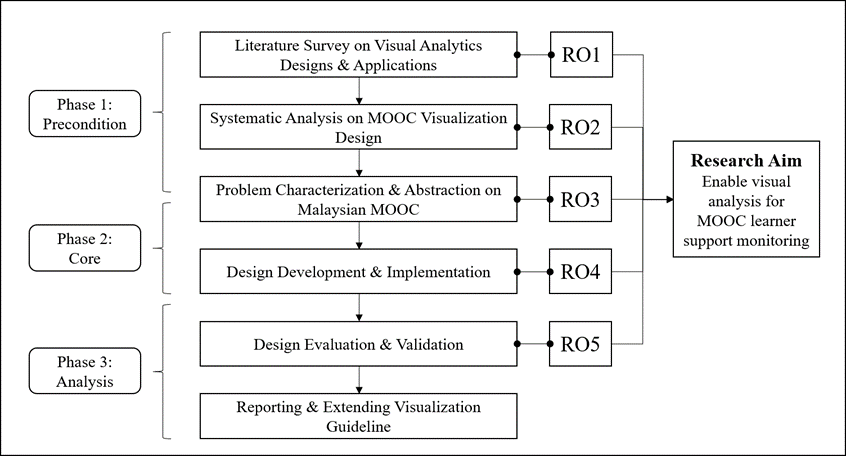
\includegraphics[scale=1]{Fig1.1}
\caption{Research framework of this study}
\label{framework} % to give the figure you want to reference a marker
\end{figure}

\medskip

\begin{enumerate}
\item A comprehensive literature survey and analysis of the recent visual analytics advances are undertaken to identify the current state of visual analytics designs and applications referring to scholarly digital libraries, particularly Scopus, IEEE Xplore, and ACM DL. This study also examines and classifies recent advances based on applied domains, design features, information-seeking tasks, data properties, data sources, and visualization techniques. The most significant design problems are identified to be addressed in this study.
\item The highlighted design problems are further investigated and verified its significance by further exploring the visualization design space of visual analytics designs and applications for MOOC data. A systematic analysis on existing MOOC visualization design is carried out by examining the reported analytic tasks, design requirements, data dimensions, visualization, and evaluation method. The resulting review helps elicit the visualization design  
\end{enumerate}

\begin{figure}[hbt!]
\centering
\begin{minipage}{0.3\textwidth}
\centering

\includegraphics[width=\linewidth]{green}
\subcaption{First subfigure}
\end{minipage}
%
\hspace{1cm}
%
\begin{minipage}{0.3\textwidth}
\centering
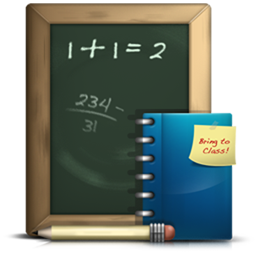
\includegraphics[width=\linewidth]{school}
\subcaption{Second subfigure}
\end{minipage}
\caption{An example with several subfigures}
\end{figure}
